\indent En esta secci\'on se muestran los tiempos de ejecuci\'on de cada algoritmo comparandose las implementaciones hechas en \textbf{C} contra las implementaciones hechas en \textbf{ASM}.\\
Dichos resultados se corresponden con la cantidad de ticks del procesador que cada algoritmo tom\'o, usando para ello el par\'ametro \textbf{-t} del programa principal, cuyo valor devuelto es justamente la cantidad de ticks para ejecutar el filtro de entrada una cantidad de veces equivalente a la pasada como par\'ametro.\\
\indent Como medimos los ticks del procesador? Es algo que se hace internamente en el c\'odigo que la c\'atedra nos proporcion\'o pero de todas formas sabemos que esto se lleva a cabo usando la instrucci\'on \textbf{rdtsc}, la cual obtiene el Time Stamp Counter (TSC). Dicho registro se incrementa en uno con cada ciclo del procesador, de modo que la cantidad de ciclos total equivale a la diferencia del valor despu\'es y antes de ejecutar cada filtro.\\
Notar que este registro es global y por ende cuenta ticks que todos los procesos del sistema estan consumiendo, no solo el nuestro, de modo que ser\'ia incorrecto hacer solo una medici\'on, en vez de eso hacemos 1000 y tomamos el promedio, para suavizar outliers (observaci\'on num\'ericamente muy distante al resto de los valores).

\subsection{SpeedUp}
\indent En computaci\'on paralela el \textit{speedup} refiere a cu\'anto m\'as r\'apido es un algoritmo paralelo (en nuestro caso refieren a las implementaciones en Asm que hacen uso de las instrucciones SSE) que el correspondiente algoritmo secuencial (lo que ser\'ia cada implementaci\'on en C).\\\\
Porqu\'e consideramos importante medir que tanto m\'as r\'apido es la versi\'on paralela que la secuencial? Si bien este tipo de an\'alisis excede originalmente lo pedido por la c\'atedra, nos pareci\'on razonable dar una idea de la magnitud de que tantas veces es mejor una implementaci\'on paralela que secuencial. Si bien este valor se desprende de la cantidad de ticks insumidos por cada implementaci\'on, nos pareci\'o adecuado formalizarlo usando el concepto de \textit{speedup} entre las dos implementaciones. Se calcula con la f\'ormula:\\
\begin{align}
S_{i vs j} = \dfrac{T_{i}} {T_{j}}
\end{align}
En nuestro caso, será:\\
\begin{itemize}
	\item $T_{i}$: cantidad de ticks del algoritmo en C
	\item $T_{j}$: cantidad de ticks del algoritmo en ASM
\end{itemize}


Para el análisis de benchmark generamos un script en {\ttfamily
  python} que genera imagenes al azar, de distintas dimensiones.

\subsection{Comparaciones entre C y ASM: Dependencia en tamaño}

Para un \emph{aspect ratio} 1:1, comparamos el tiempo que tarda C con
optimización -O3 y ASM en procesar cada imagen.

\subsubsection{Diferencia de Imagenes}

En la figura~\ref{fig:tiempo_diff} observamos el tiempo de
procesado, por píxel, para varias imágenes entre 100x100 y 2000x2000
píxels. 

\begin{figure}
  \centering
  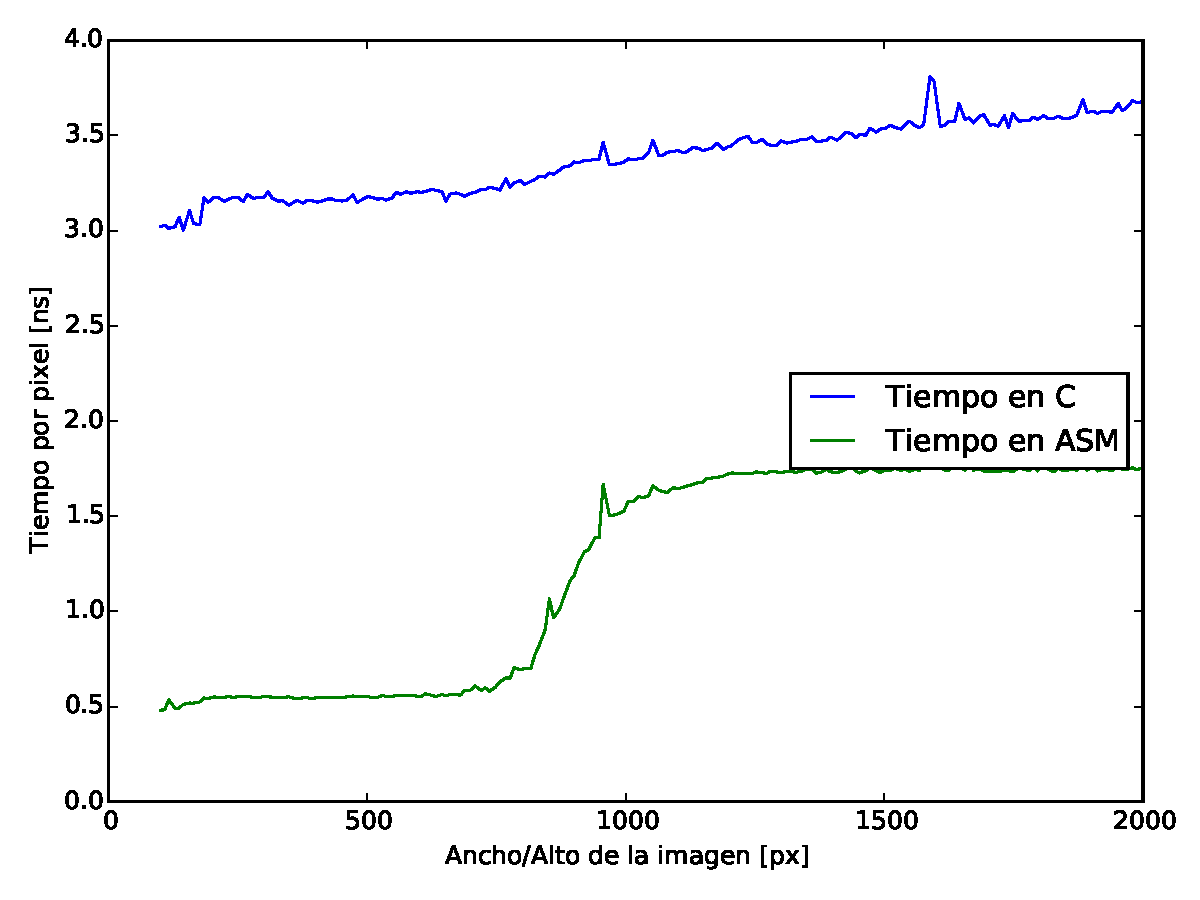
\includegraphics[width=0.7\columnwidth]{tiempo_diff.pdf}
  \caption{Tiempo por píxel para imágenes cuadradas. Observamos un
    salto, para ASM, entre 800 y 1000 píxeles.}
  \label{fig:tiempo_diff}
\end{figure}

Observamos una muy pequeña tendencia creciente en el tiempo de
procesado por píxel para la implementación en C (20\% más lento en
imágenes de 100 veces la cantidad de píxeles), mientras que en el caso
de ASM el tiempo parece ser constante entre 200 y 800 píxeles y entre
1000 y 2000, con una bastante abrupta transición en la que se triplica
el tiempo de procesado entre 800 y 1000 píxeles. Para 800x800 píxeles de
imagen, tenemos en total
$0.64\,\text{MP} \cdot 4\text{bytes/pixel} = 2.5\text{MB}$. Como son en
total tres imágenes, estamos usando $7.5\text{MB}$ de memoria, que es
el tamaño de la cache L3 del procesador utilizado. Se vuelva a
estabilizar al llegar a 1000x1000, 4MB por imagen (dos imágenes
entrarían en cache).

En la implementación de C no se observa ese comportamiento,
probablemente debido a que la optimización O3 realiza un algoritmo
\emph{cache aware}, mediante el flag {\ttfamily
  -freorder-blocks-and-partition}. Este mismo salto, y el hecho de que
suceda sólo en la implementación en ASM, implica un salto también en
el \emph{speedup}, como se ve en~\ref{fig:speedup_diff}.

\begin{figure}
  \centering
  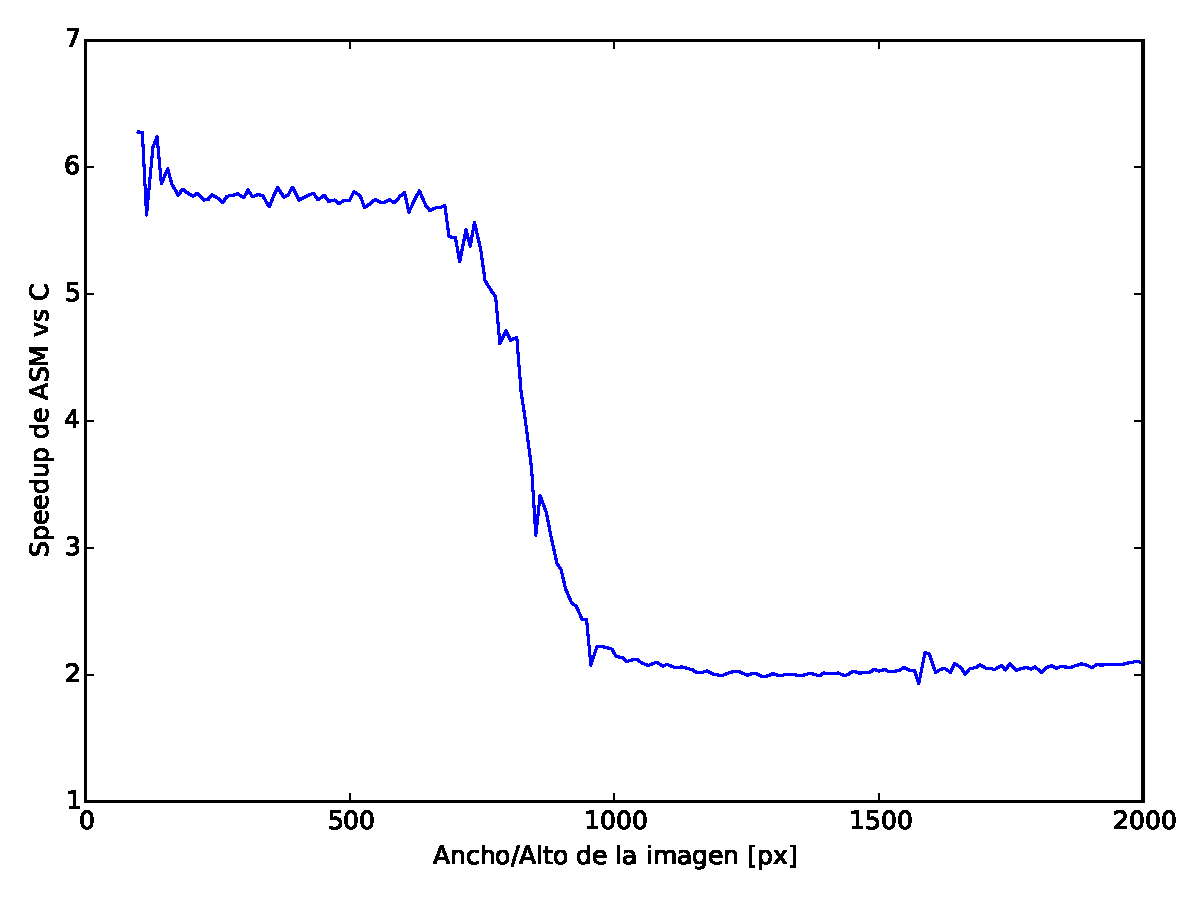
\includegraphics[width=0.7\columnwidth]{speedup_diff.pdf}
  \caption{\emph{Speedup} para imágenes cuadradas. Observamos un
    salto entre 800 y 1000 píxeles, que se traslada de la baja de
    performance en el código de ASM}
  \label{fig:speedup_diff}
\end{figure}


\subsubsection{Blur Gaussiano}

En la figura~\ref{fig:tiempo_blur} observamos el tiempo de
procesado, por píxel, para varias imágenes entre 100x100 y 2000x2000
píxels. 

\begin{figure}
  \centering
  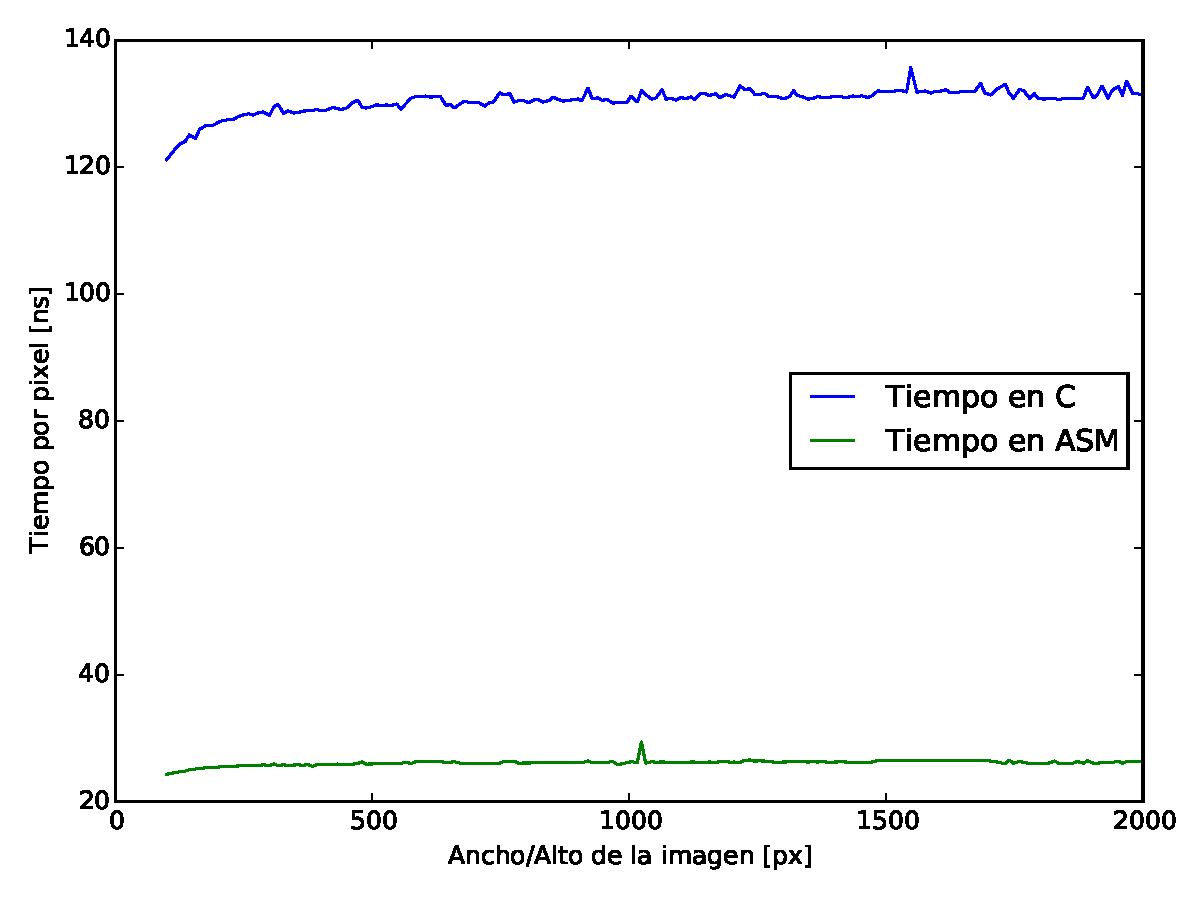
\includegraphics[width=0.7\columnwidth]{tiempo_blur.pdf}
  \caption{Tiempo por píxel para imágenes cuadradas. Observamos un
    comportamiento creciente, que se estabiliza a partir de
    $\approx 300$ px.}
  \label{fig:tiempo_blur}
\end{figure}

En este gráfico vemos que ambos algoritmos arrancan con una tendencia
creciente hasta los 300 px, a partir del cual el tiempo por píxel se
mantiene constante. Que ambos sean de la misma tendencia se corrobora
en el estudio del \emph{speedup}, en el que se ve que se mantiene
uniforme para todos los tamaños de la imagen.

\begin{figure}
  \centering
  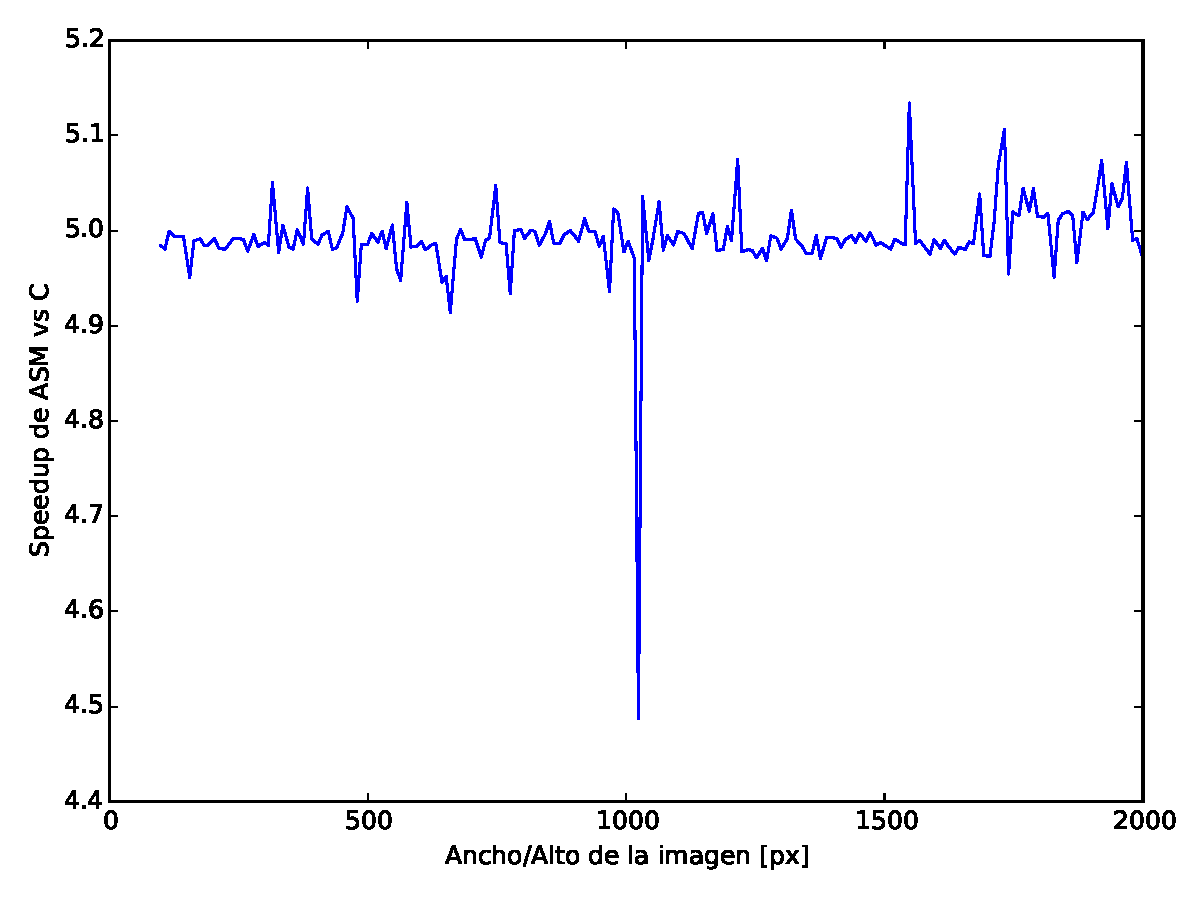
\includegraphics[width=0.7\columnwidth]{speedup_blur.pdf}
  \caption{\emph{Speedup} para imágenes cuadradas. Observamos un
    comportamiento uniforme de 5x.}
  \label{fig:speedup_blur}
\end{figure}


\subsection{Comparaciones entre C y ASM: Dependencia en aspect ratio}

En este caso, mantuvimos el tamaño de la imagen constante y variamos
el aspect ratio. No se observó ninguna dependencia en ninguno de los
casos, como se puede ver en las figuras~\ref{fig:tiempo_ratio_diff},
~\ref{fig:speedup_ratio_diff}, ~\ref{fig:tiempo_ratio_blur},
~\ref{fig:speedup_ratio_blur}.

\begin{figure}
  \centering
  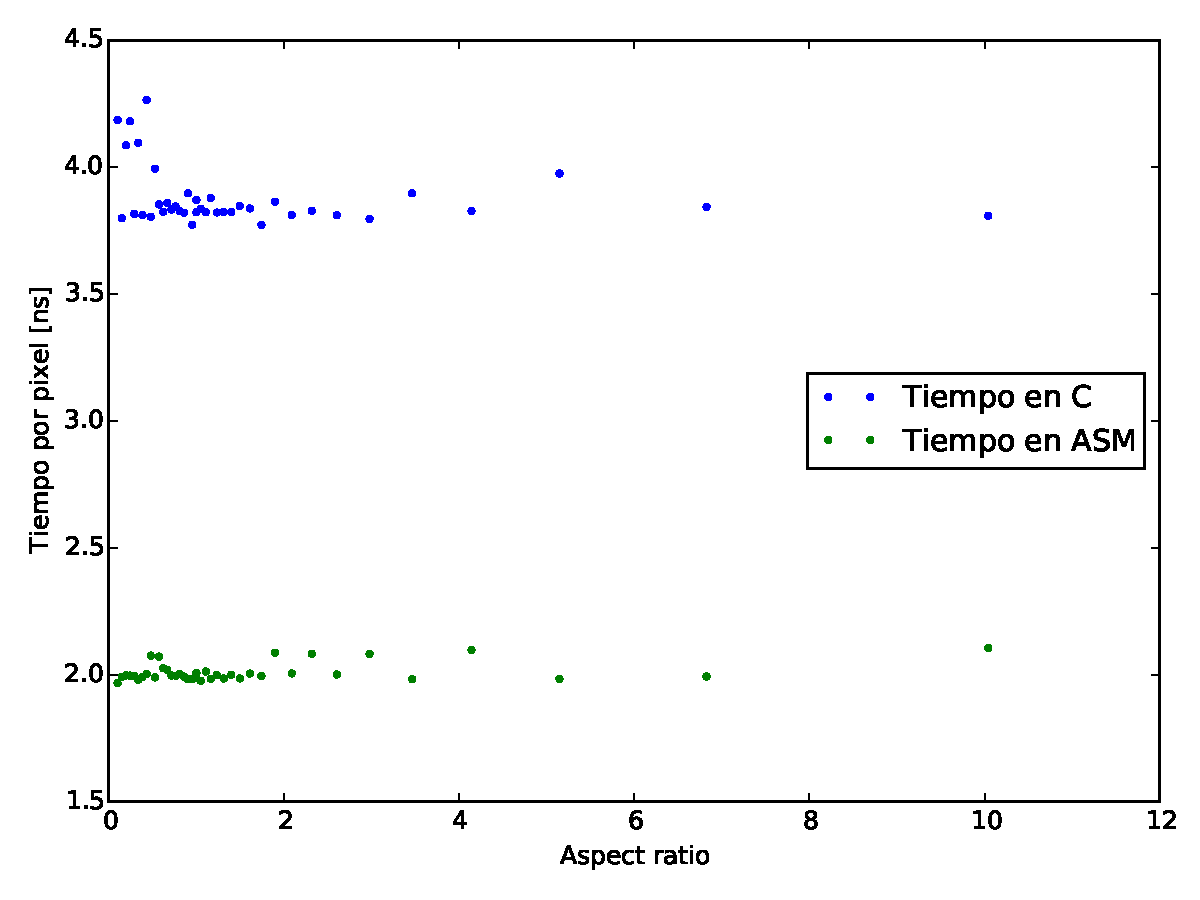
\includegraphics[width=0.7\columnwidth]{tiempo_ratio_diff.pdf}
  \caption{Tiempo de procesado por píxel para distintos aspect ratio
    con filtro diff.}
  \label{fig:tiempo_ratio_diff}
\end{figure}

\begin{figure}
  \centering
  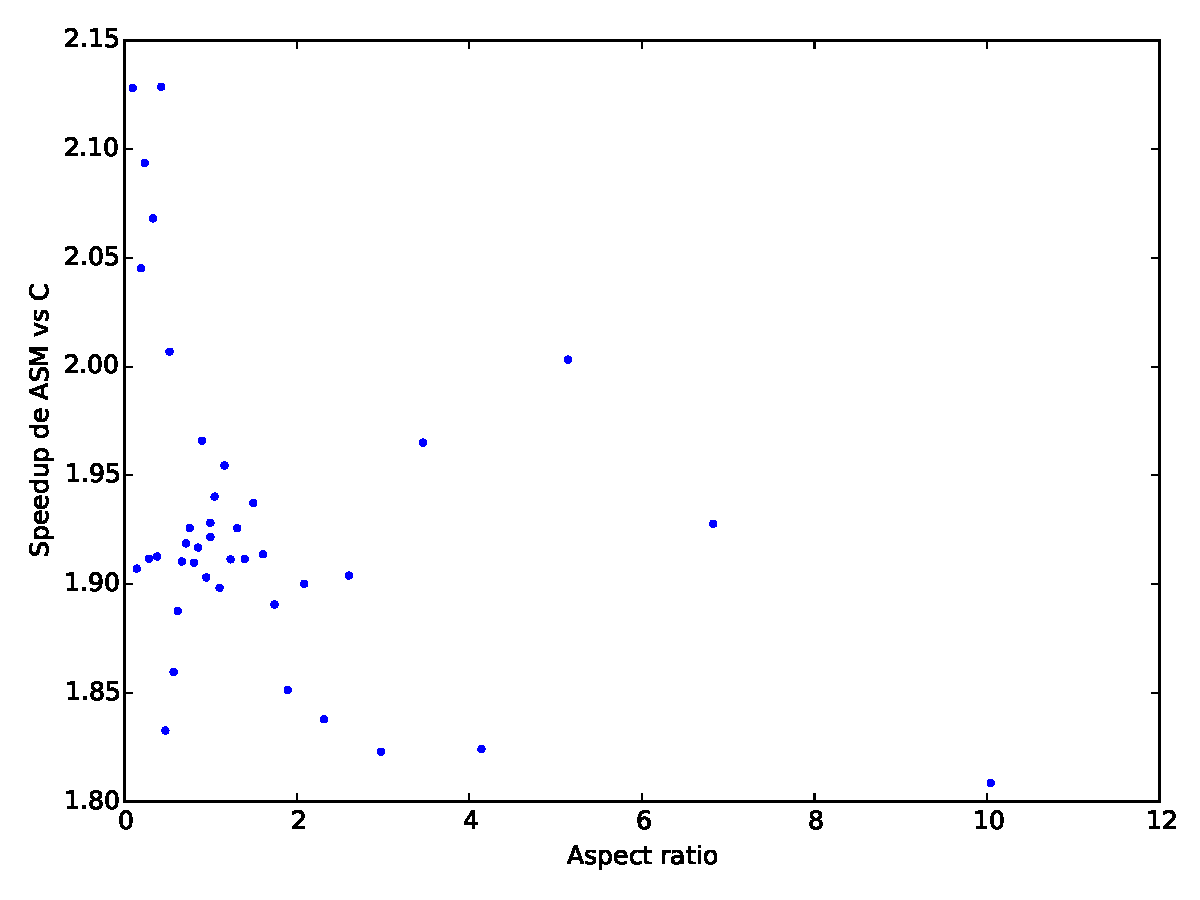
\includegraphics[width=0.7\columnwidth]{speedup_ratio_diff.pdf}
  \caption{\emph{Speedup} de procesado por píxel para distintos aspect
    ratio con filtro diff.}
  \label{fig:speedup_ratio_diff}
\end{figure}

\begin{figure}
  \centering
  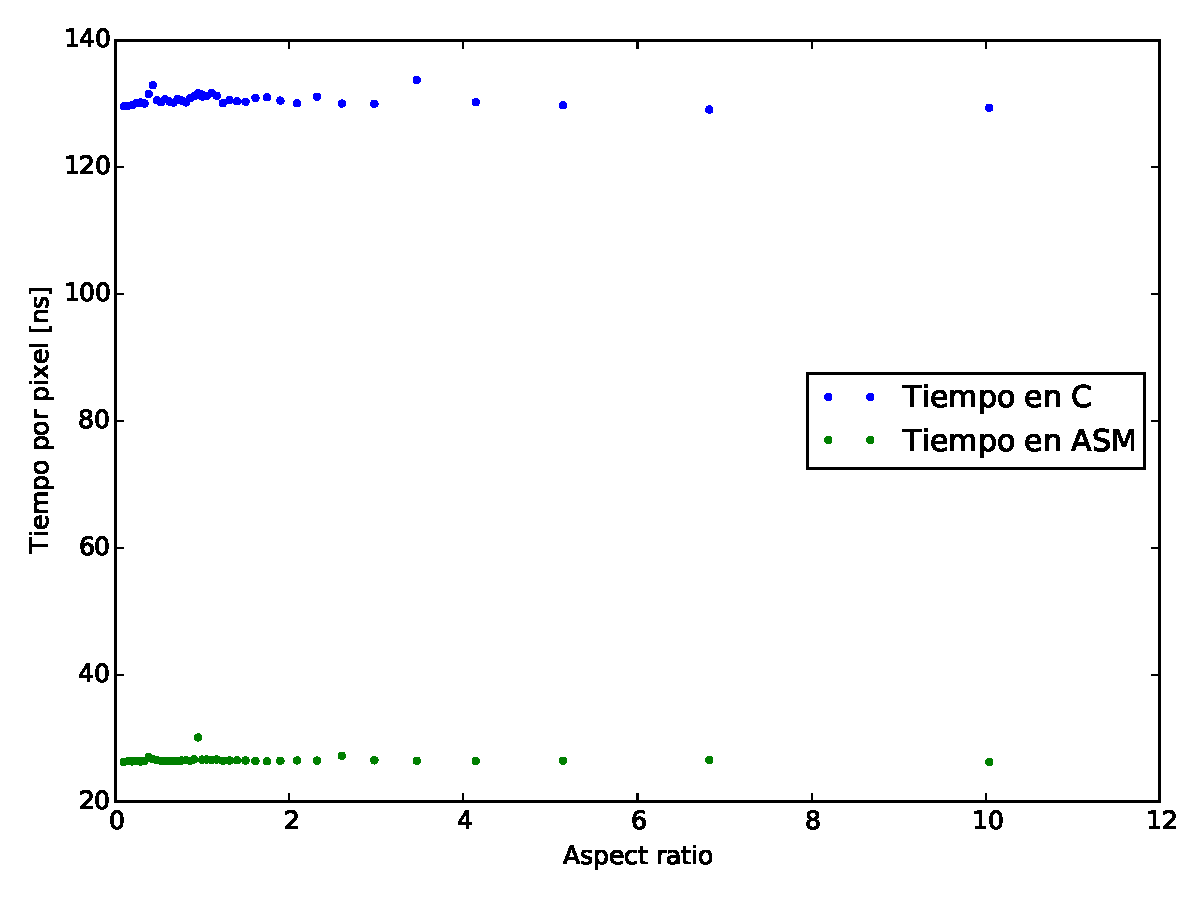
\includegraphics[width=0.7\columnwidth]{tiempo_ratio_blur.pdf}
  \caption{Tiempo de procesado por píxel para distintos aspect ratio
    con filtro blur.}
  \label{fig:tiempo_ratio_blur}
\end{figure}

\begin{figure}
  \centering
  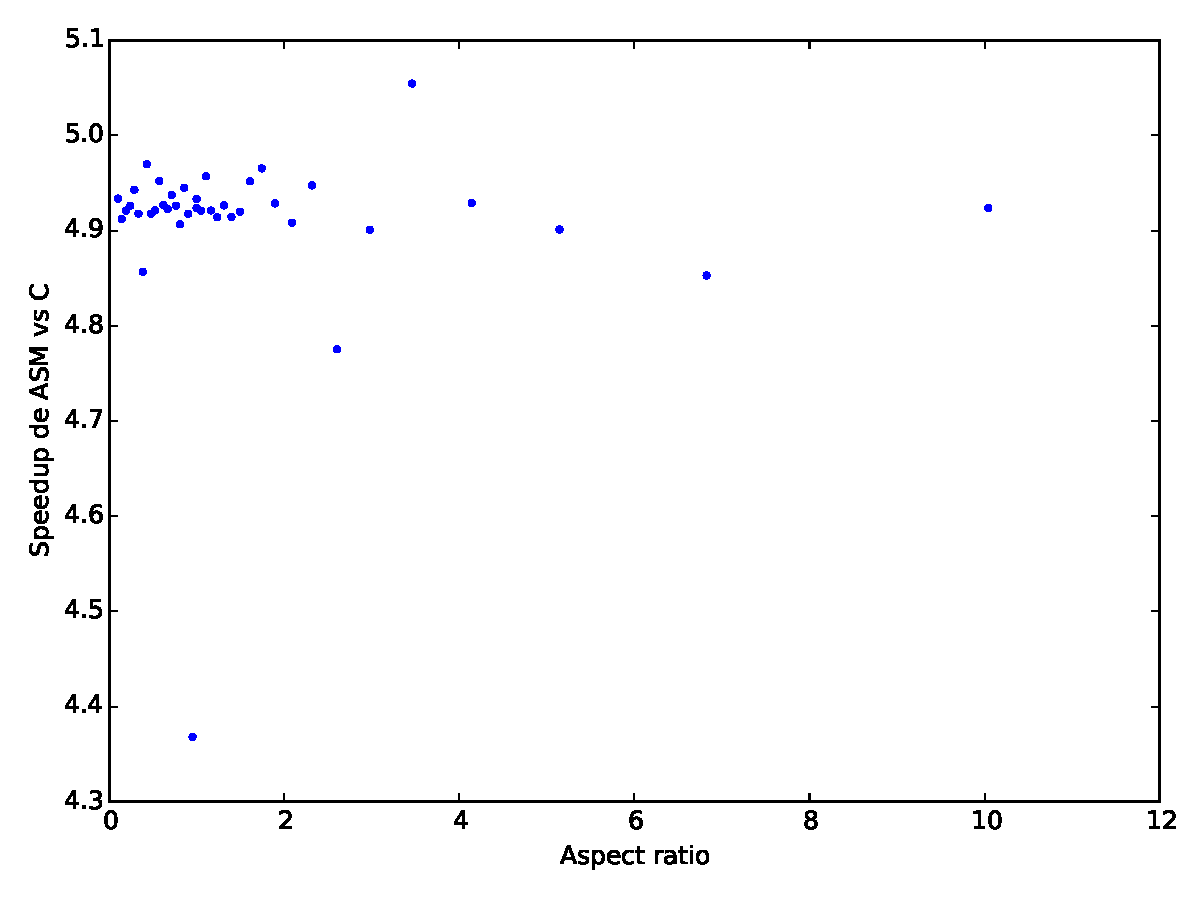
\includegraphics[width=0.7\columnwidth]{speedup_ratio_blur.pdf}
  \caption{\emph{Speedup} de procesado por píxel para distintos aspect ratio
    con filtro blur.}
  \label{fig:speedup_ratio_blur}
\end{figure}

\subsection{Comparaciones entre C y ASM: Dependencia con el radio de
  blur}

Finalmente, observamos en la figura~\ref{fig:tiempo_radio} el tiempo
de procesado por píxel para distintos radios.

\begin{figure}
  \centering
  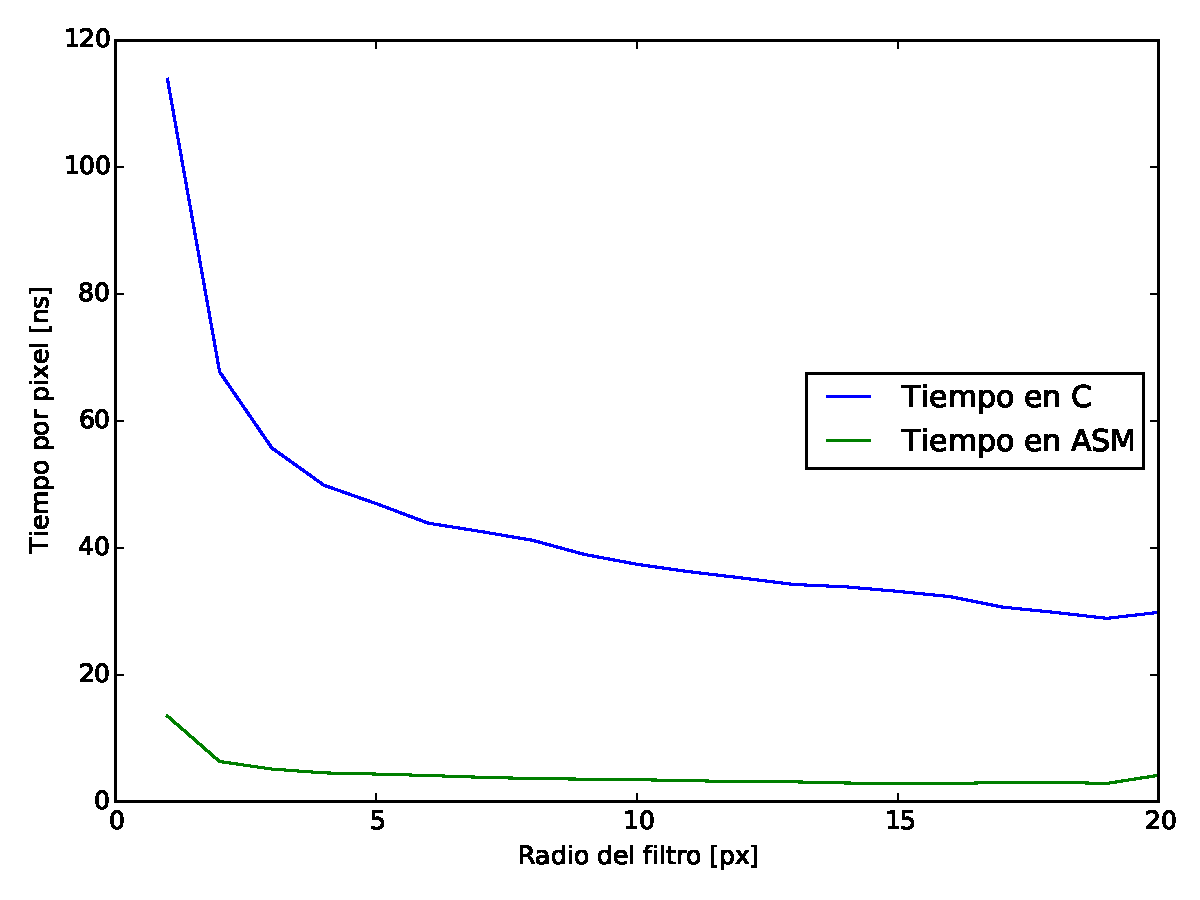
\includegraphics[width=0.7\columnwidth]{tiempo_radio_blur.pdf}
  \caption{Tiempo de procesado por píxel para distintos radios
    con filtro blur.}
  \label{fig:tiempo_radio_blur}
\end{figure}

\begin{figure}
  \centering
  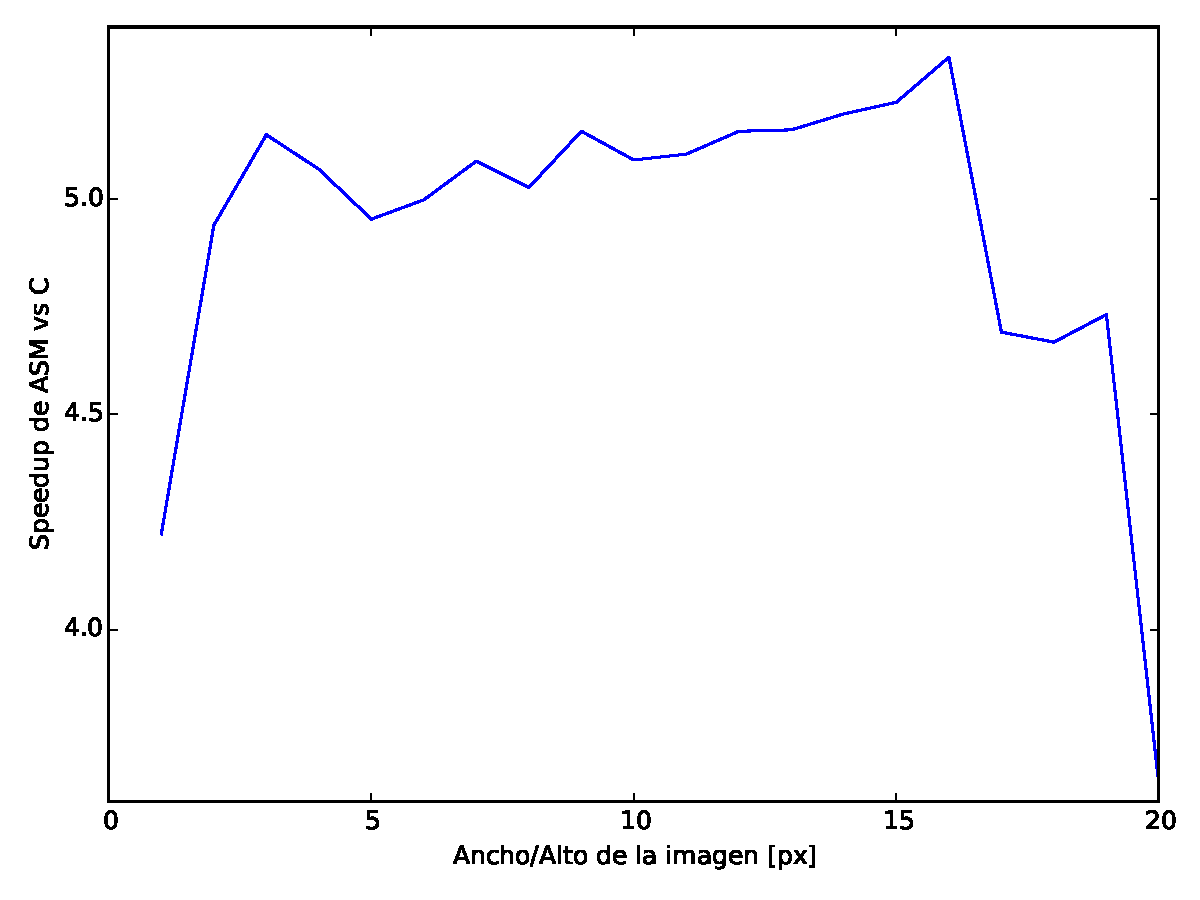
\includegraphics[width=0.7\columnwidth]{speedup_radio_blur.pdf}
  \caption{\emph{Speedup} de procesado por píxel para distintos radios
    con filtro blur.}
  \label{fig:speedup_radio_blur}
\end{figure}

\subsection{Comparaciones entre C -O0 y C -O3: Filtro de diferencias}

\begin{figure}
  \centering
  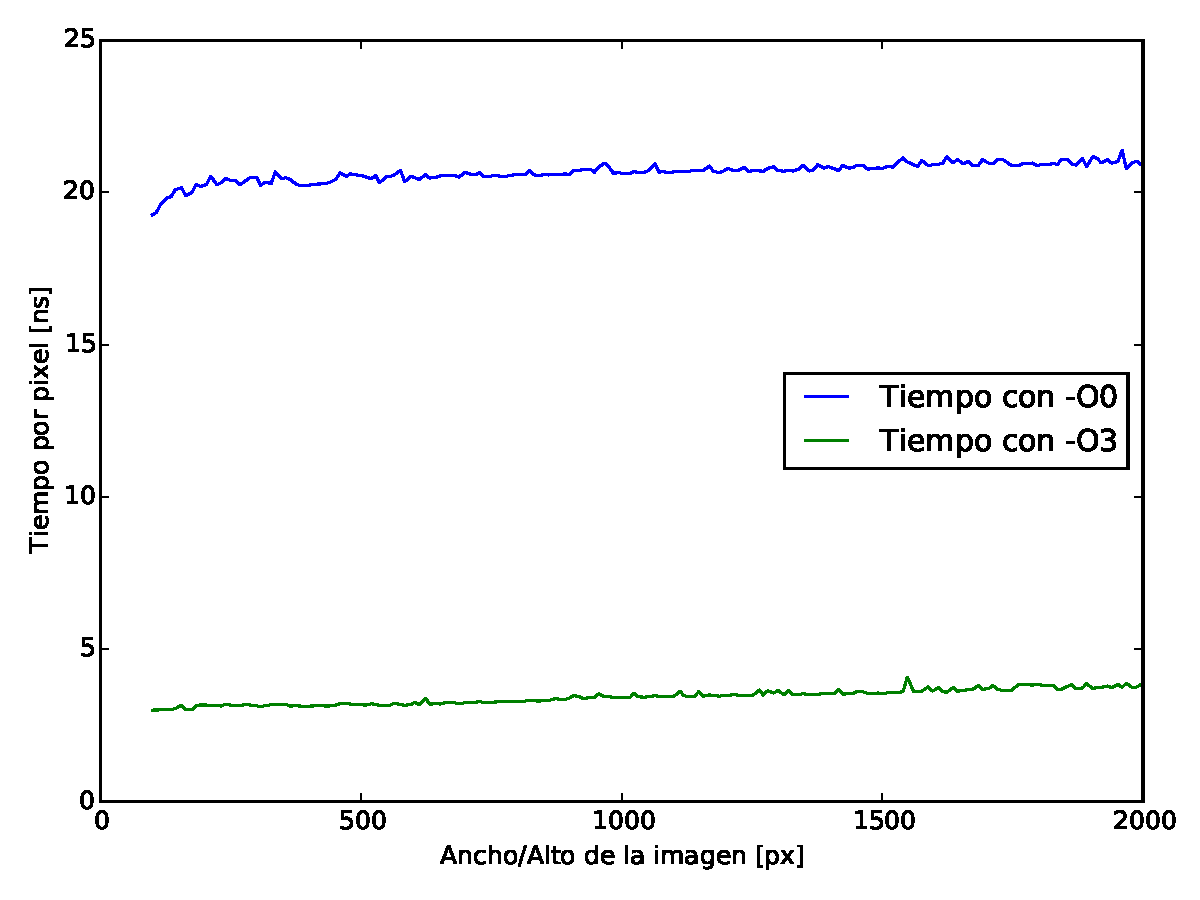
\includegraphics[width=0.7\columnwidth]{tiempo_optimiz_diff.pdf}
  \caption{Tiempo de procesado por píxel para distintos tamaños.}
  \label{fig:tiempo_optimiz_diff}
\end{figure}

\begin{figure}
  \centering
  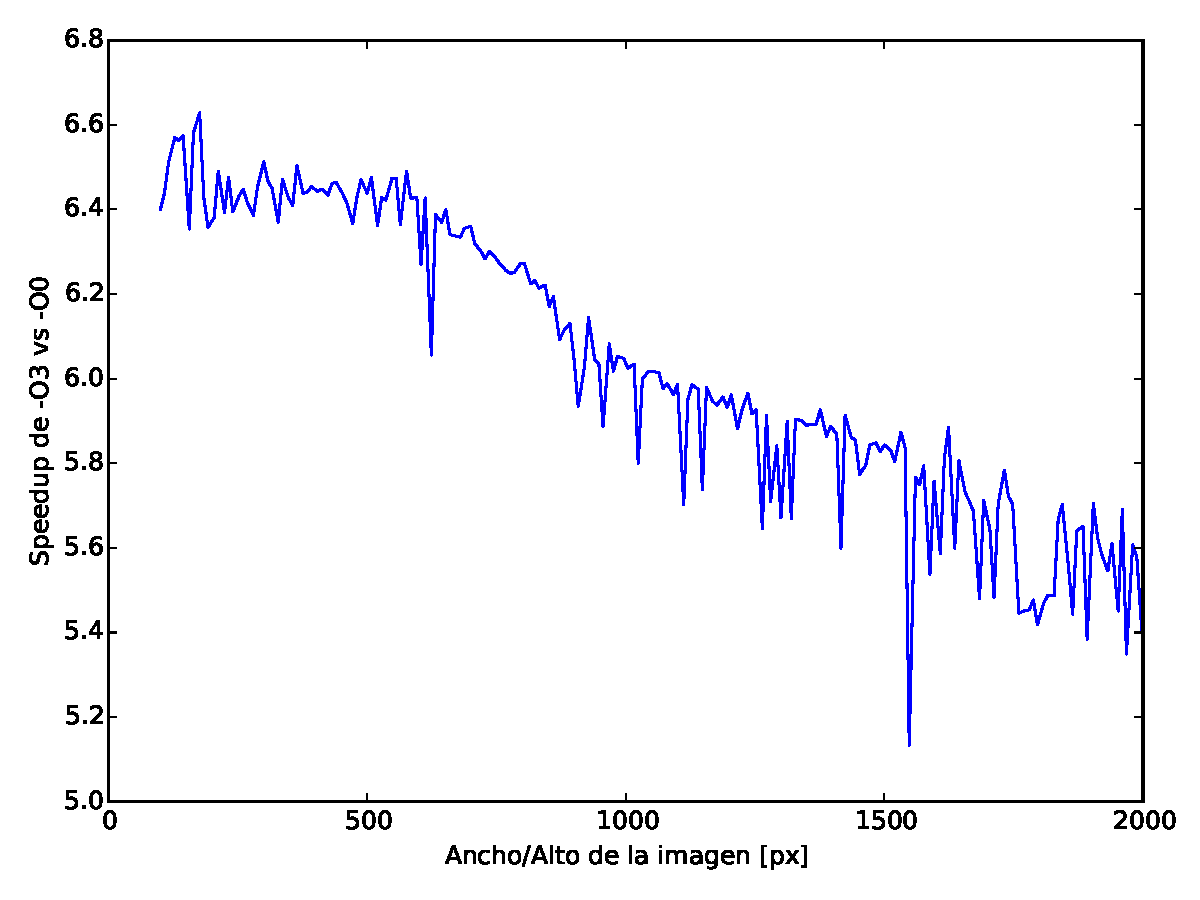
\includegraphics[width=0.7\columnwidth]{speedup_optimiz_diff.pdf}
  \caption{\emph{Speedup} de procesado por píxel para distintos tamaños.}
  \label{fig:speedup_optimiz_diff}
\end{figure}


  
\subsection{Algunas conclusiones}

A partir de los resultados y tablas vistas podemos mencionar las siguientes conclusiones generales que aplican a todos los filtros:
  \begin{itemize}
    \item Las implementaciones hechas en \textit{Assembler} son efectivamente m\'as r\'apidas que las implementaciones hechas en \textit{C}. Esto era lo esperado pue\'es las implementaciones en \textit{Assembler} hacen uso de las instrucciones SSE y se procesan mas de un pixel simultaneamente.
    \item En los algoritmos en los que no hubo conversi\'on a Float de los datos, la velocidad de resoluci\'on fue mayor porque al no ser necesario usar floats, cada pixel ocupaba menos bytes y por ende pod\'iamos procesar mayor cantidad simultaneamente. 
	\item El SpeedUp de las funciones no cambi\'o demasiado entre las funciones. 
	Y todas estas operaciones se pueden obtener directamente con instrucciones SIMD, mientras que en C hubo que programarlas, realentizando el algoritmo.
	\item En los gr\'aficos de SpeedUp se pueden ver picos, que si bien no son muy marcados, llaman	la atenci\'on. Pensamos que esto puede suceder porque medimos los ciclos que tarda el procesador en correr las funciones, y estos se pueden ver afectados por otro uso en simult\'aneo que se le est\'e dando al mismo. 
    \item En todos los gr\'aficos de comparacion entre C y ASM las curvas presentan un crecimiento semejante al de una funcion cuadr\'atica. Esto se debe a que la escala tomada en el eje de abscisas hace referencia al tama\~no de un lado de las imagenes (todas las imagenes son cuadradas). Como la cantidad total de pixeles en la imagen es el cuadrado de este valor, la cantidad de ciclos de cpu aumenta linealmente respecto a la cantidad de pixeles.
   \end{itemize}
  






